\documentclass{article}

\usepackage{graphicx}
\usepackage{tikz}
\usepackage{tikzsymbols}
\usetikzlibrary{calc}
\usepackage{float}
\usepackage{pdflscape}

\def\centerarc[#1](#2)(#3:#4:#5){\draw[#1] ($(#2)+({#5*cos(#3)},{#5*sin(#3)})$) arc (#3:#4:#5);}

\pagestyle{empty}
\begin{document}
	\centering
	\begin{figure}[H]
			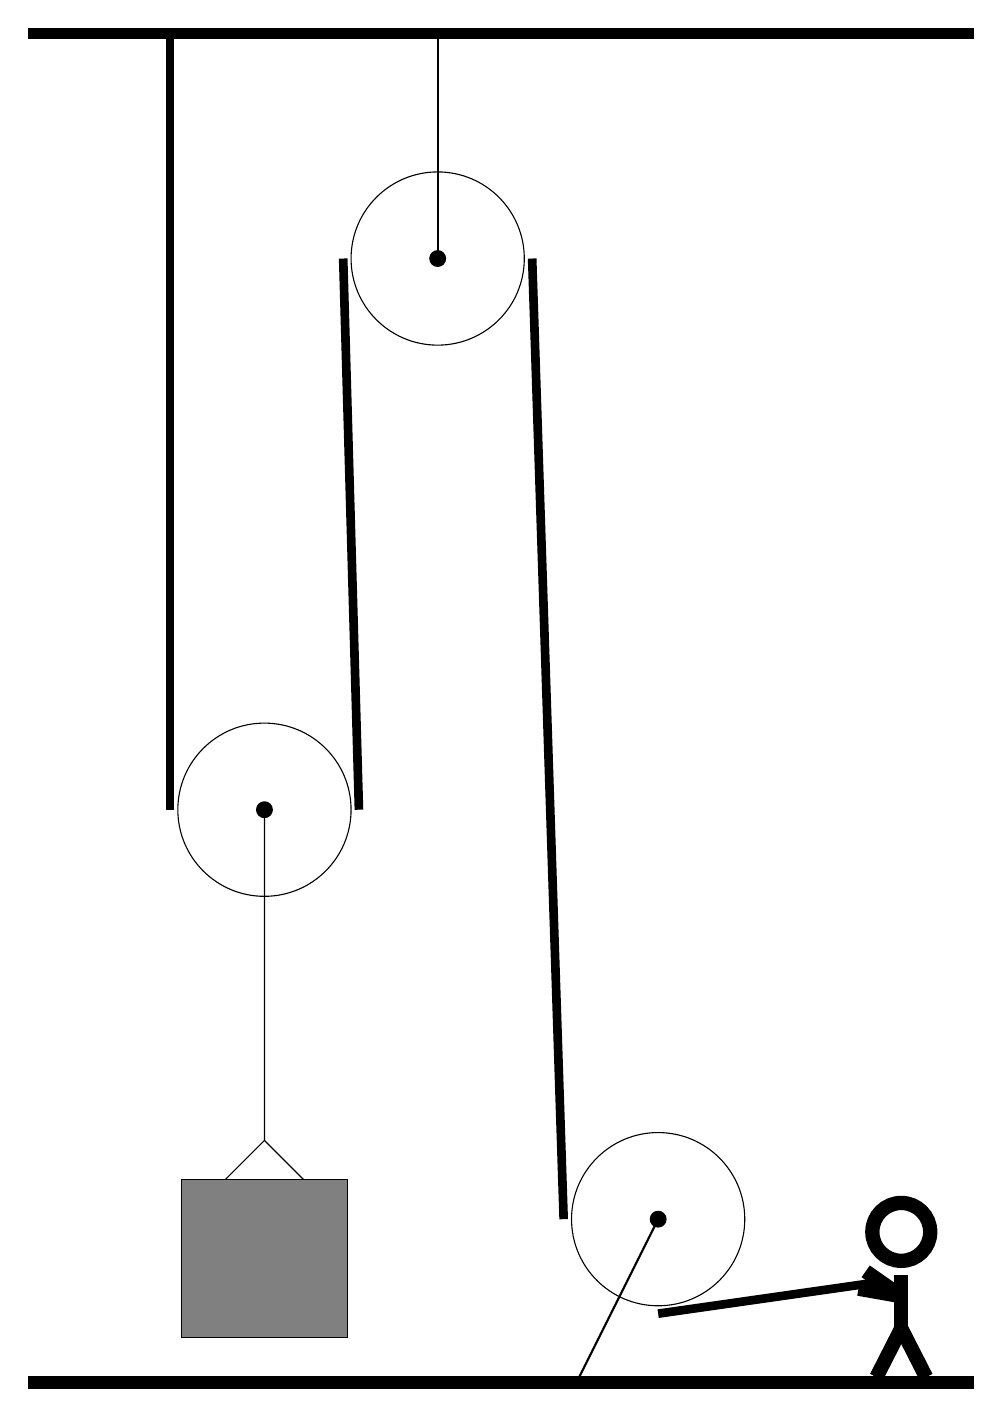
\begin{tikzpicture}
				%%%%% START %%%%%
				\def\a{14}
				\def\radlg{1.1}
				\def\radrp{1.2000000000000002}
				\def\radsm{0.1}
				\def\yone{\a-\a*0.7}
				\def\xone{1}
				\def\ytwo{\a-\a*0.2}
				\def\xtwo{3.2}
				\def\ythree{-1}
				\def\xthree{6}
				\def\dx{9}
				\def\dy{-1.90}
				\def\dw{1.75mm}
				\def\width{1.1mm}
				
				\draw[fill=black] (-2,\a) rectangle (10,\a+0.125);
				
				\draw (\xtwo,\ytwo) circle (\radlg);
				\draw[fill=black] (\xtwo,\ytwo) circle (\radsm);
				\draw[thick] (\xtwo,\ytwo) -- (\xtwo,\a);
				
				\draw (\xthree,\ythree) circle (\radlg);
				\draw[fill=black] (\xthree,\ythree) circle (\radsm);
				\draw[thick] (\xthree,\ythree) -- (\xthree-1,-3);
				
				\draw (\xone,\yone) circle (\radlg);
				\draw[fill=black] (\xone,\yone) circle (\radsm);
				
				\draw (\xone,\yone) -- (\xone,\a-\a) -- (\xone-0.5,\a-\a-0.5);
				\draw (\xone,\a-\a) -- (\xone+0.5,\a-\a-0.5);
				\draw[fill=black!50] (\xone-1.05,\a-\a-0.5) rectangle (\xone+1.05,\a-\a-2.5);  
				
				\draw[line width=\width] (\xone-\radrp,\a) -- (\xone-\radrp,\yone); 
				\centerarc[line width=\width](\xone,\yone)(180:360:\radrp);
				\draw[line width=\width](\xone+\radrp,\yone) -- (\xtwo-\radrp,\ytwo);
				\centerarc[line width=\width](\xtwo,\ytwo)(0:180:\radrp);				
				\draw[line width=\width](\xtwo+\radrp,\ytwo) -- (\xthree-\radrp,\ythree);
				\centerarc[line width=\width](\xthree,\ythree)(180:270:\radrp);
				\draw[line width=\width](\xthree,\ythree-\radrp) -- (\dx-0.2,\dy+0.1);

				\node at (\dx,\dy) {\Strichmaxerl[10][-35][170]};
				
				\draw[fill=black] (-2,-3) rectangle (10,-3.15);
				%%%%% END %%%%%
			\end{tikzpicture}
	\end{figure}
	
\end{document}